%
%
\documentclass{article}
\usepackage{amsmath}
\usepackage{graphicx}
\usepackage{color}
\usepackage{caption}
\usepackage{amsfonts}
\usepackage[margin=2.5cm,bmargin=.5cm]{geometry}
\setlength{\voffset}{-2cm}
%\usepackage{tikz}
\newcommand{\bs}{\boldsymbol}                               %

\begin{document}

\title{Sample graphs}
\author{Dominic Skinner}
\pagenumbering{gobble}
\maketitle
This short document is just to show the graphs that can be
currently be produced by the existing matlab code. 
\begin{figure}[ht]\centering
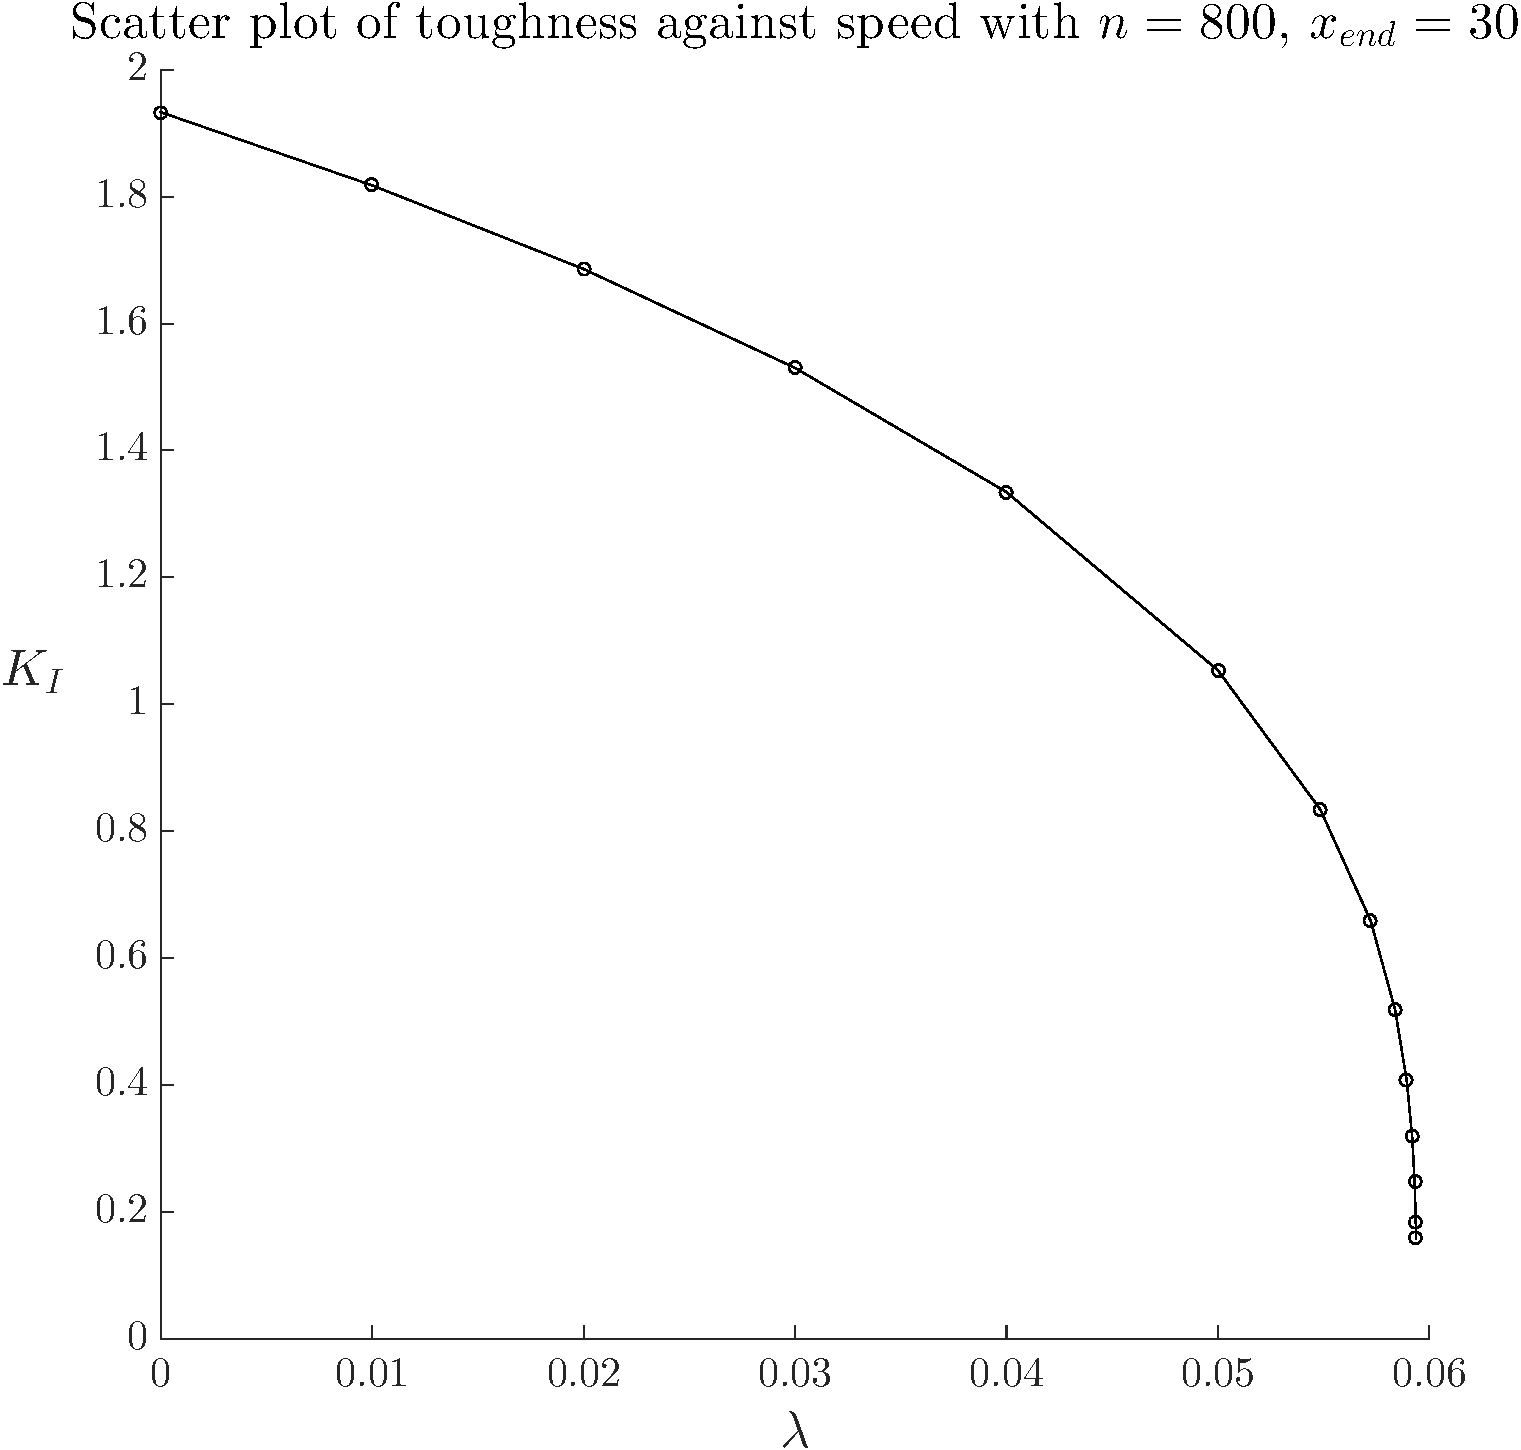
\includegraphics[scale=0.36]{K-lambda.pdf}
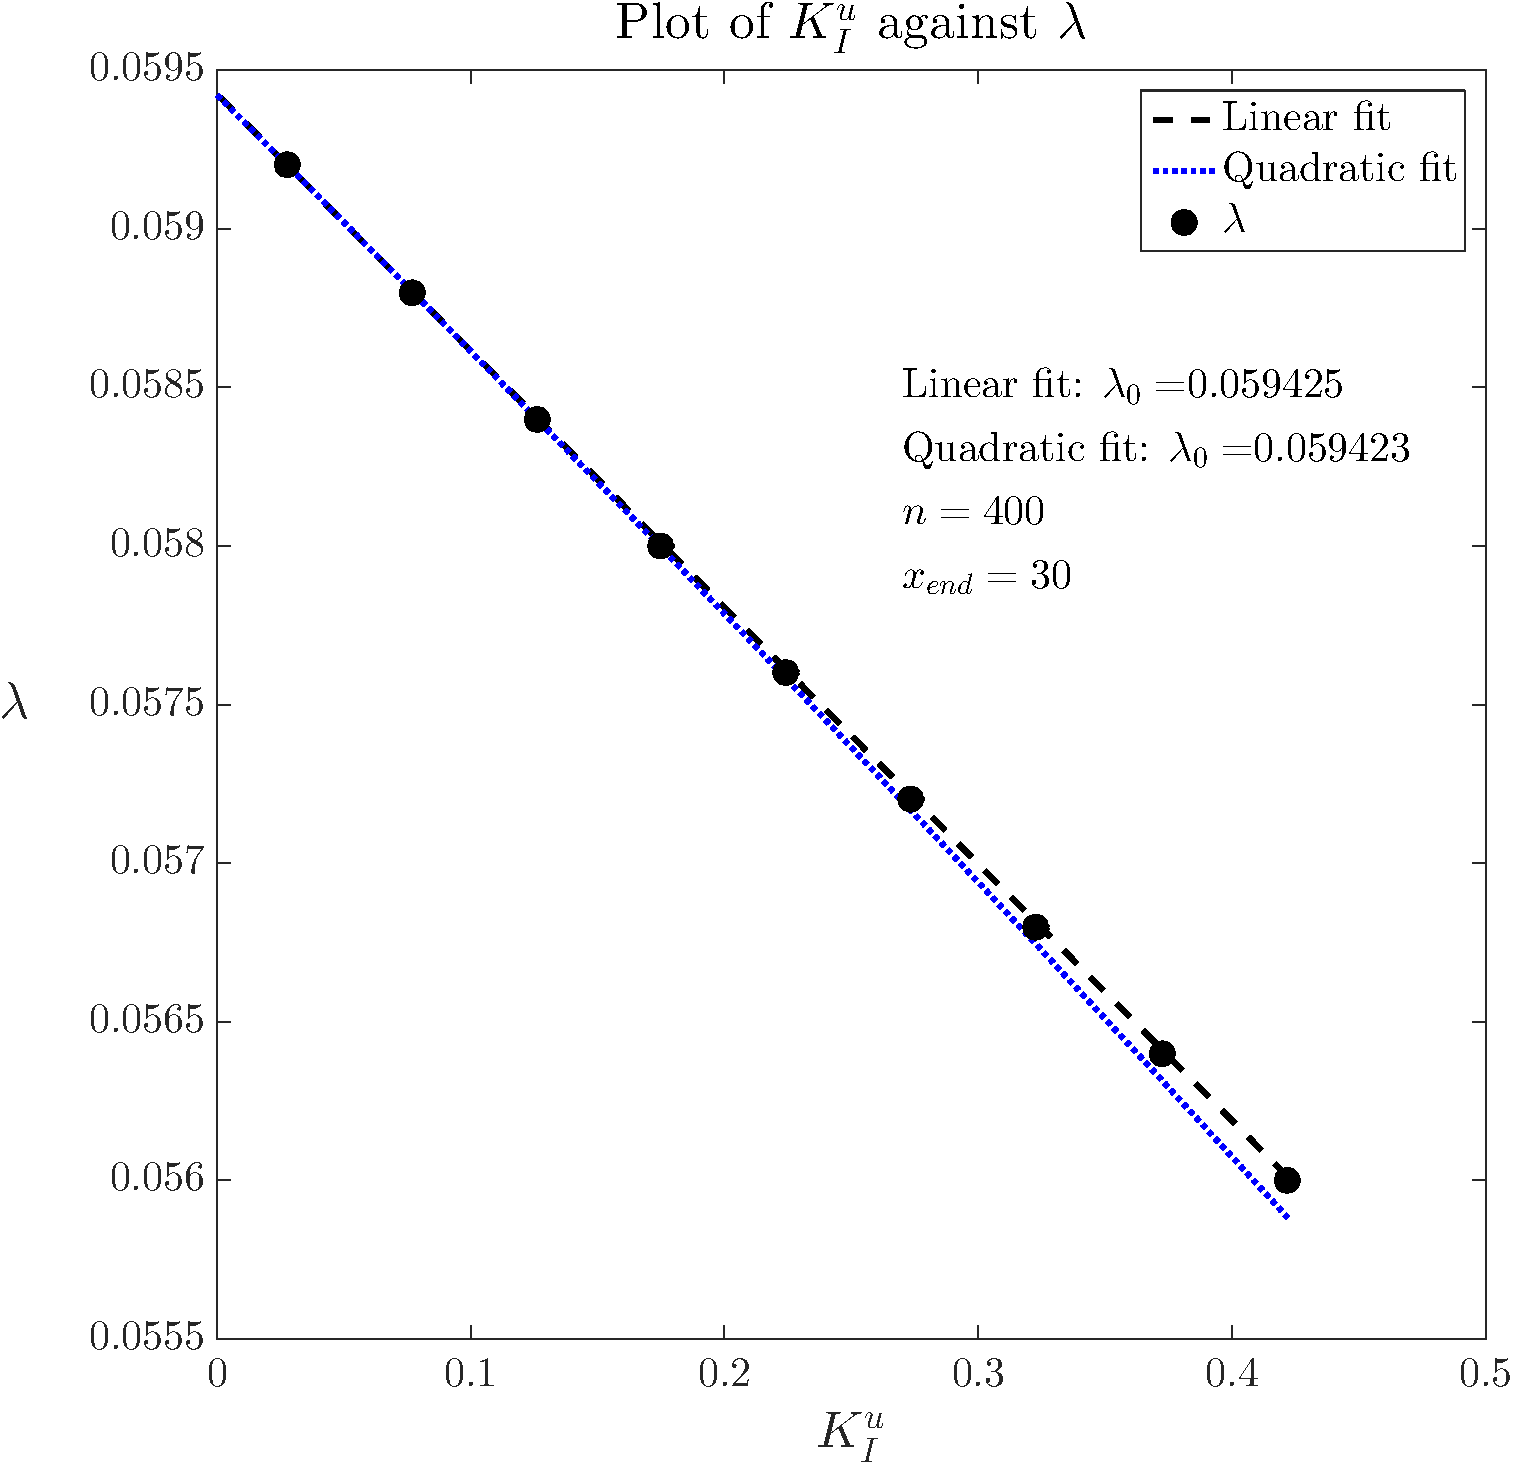
\includegraphics[scale=0.38]{l0.pdf}
\end{figure}
%
\begin{figure}[!ht]\centering

\includegraphics[scale=0.50]{hprime-x.pdf}
\\[8pt]
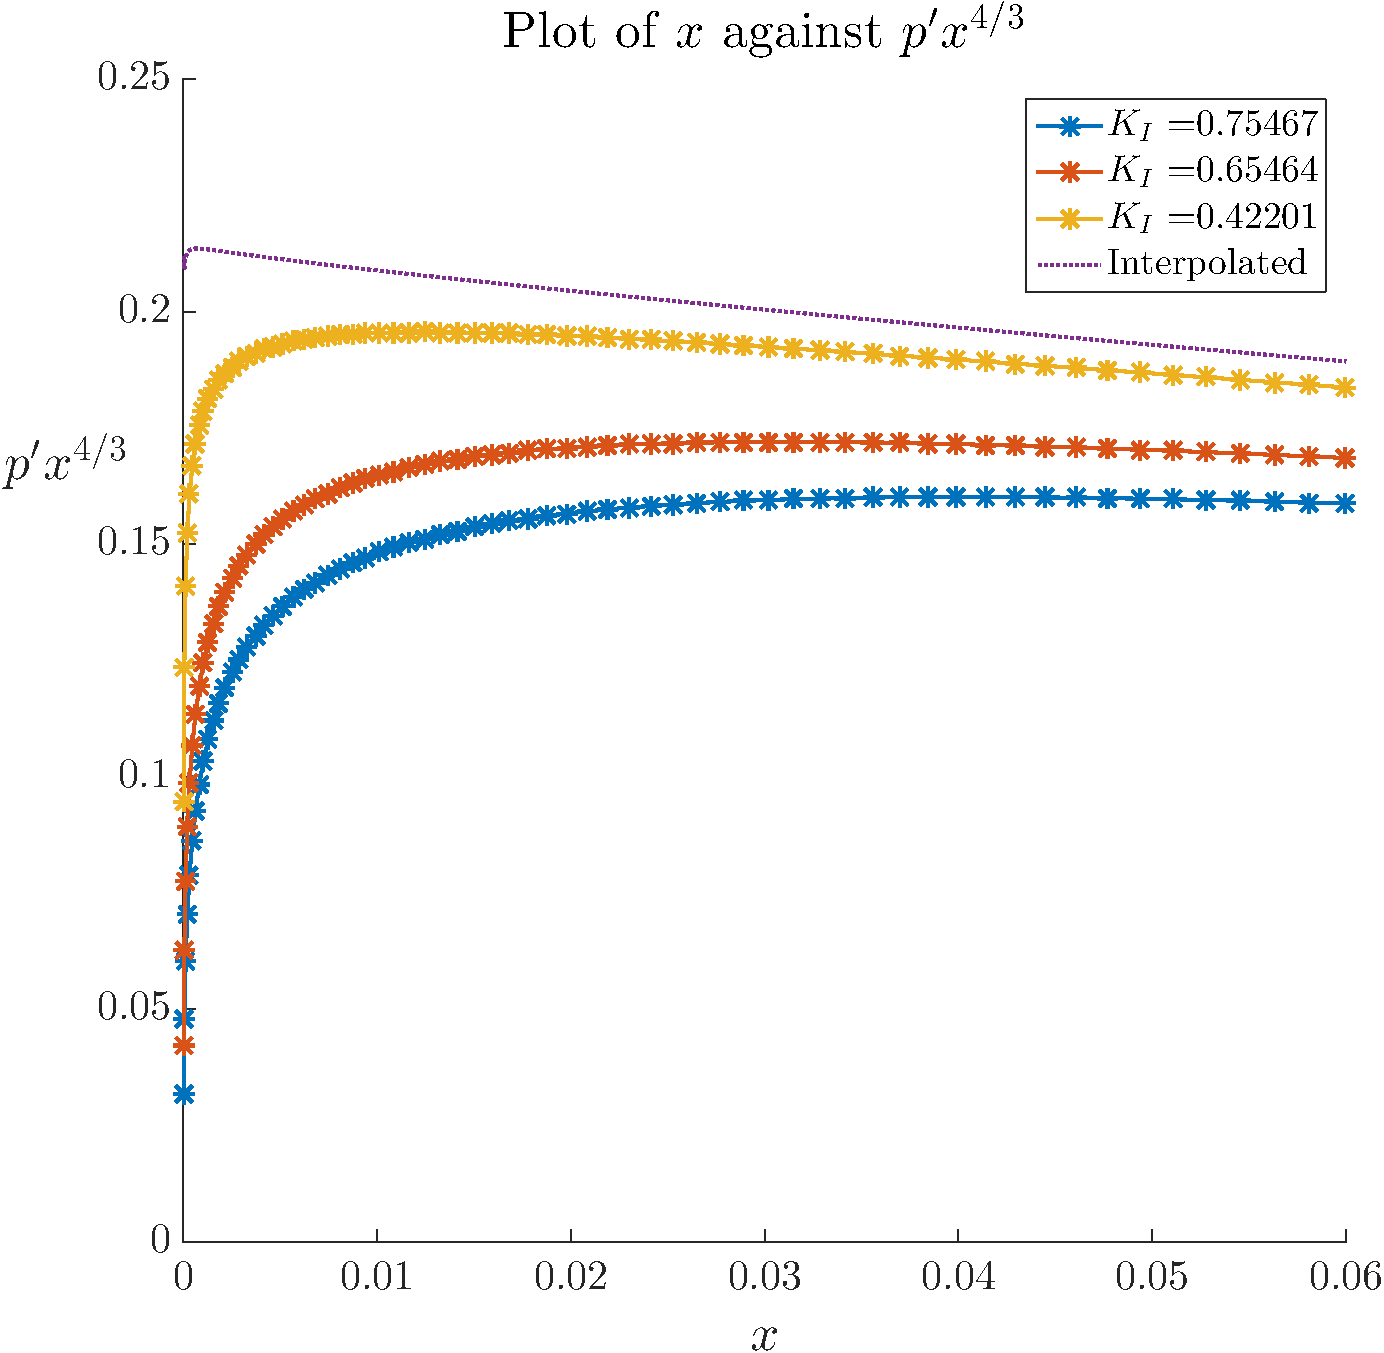
\includegraphics[scale=0.50]{pprime-x.pdf}
\end{figure}
%
\begin{figure}[!ht]\centering
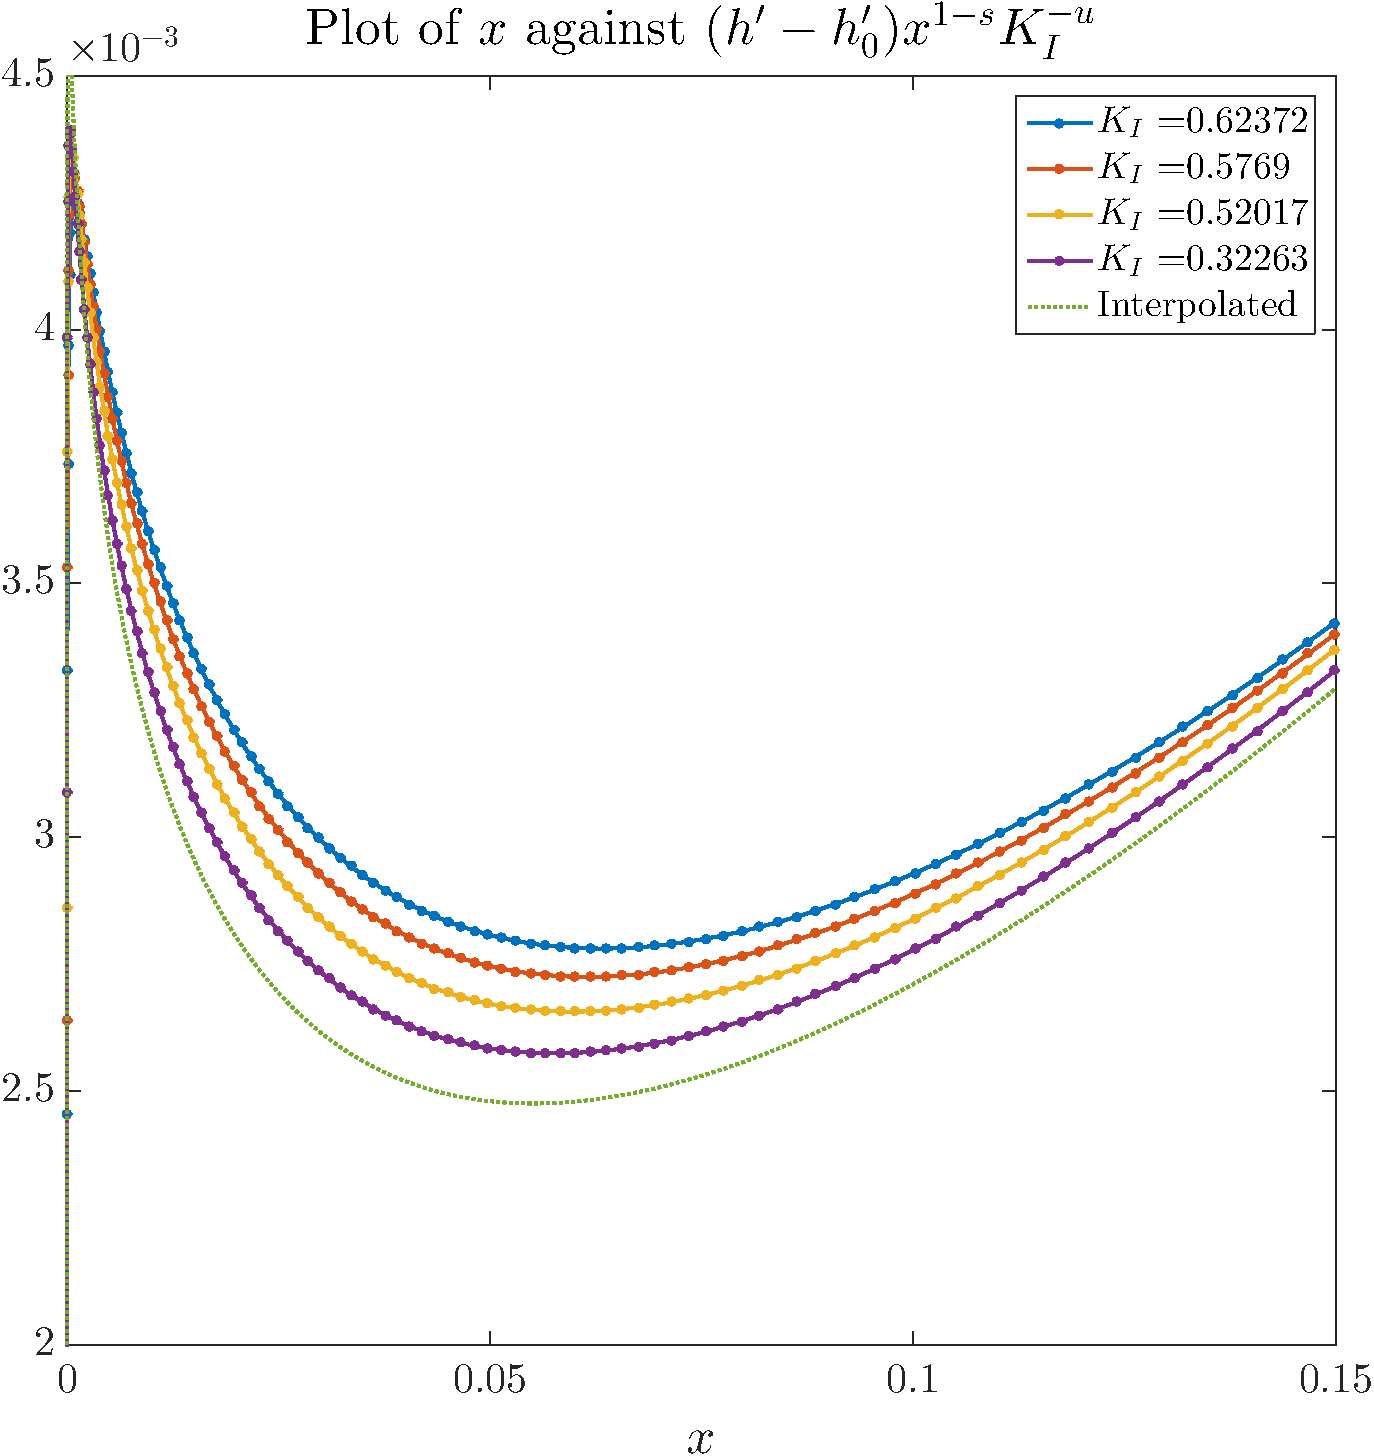
\includegraphics[scale=0.5]{h1-prime.pdf}
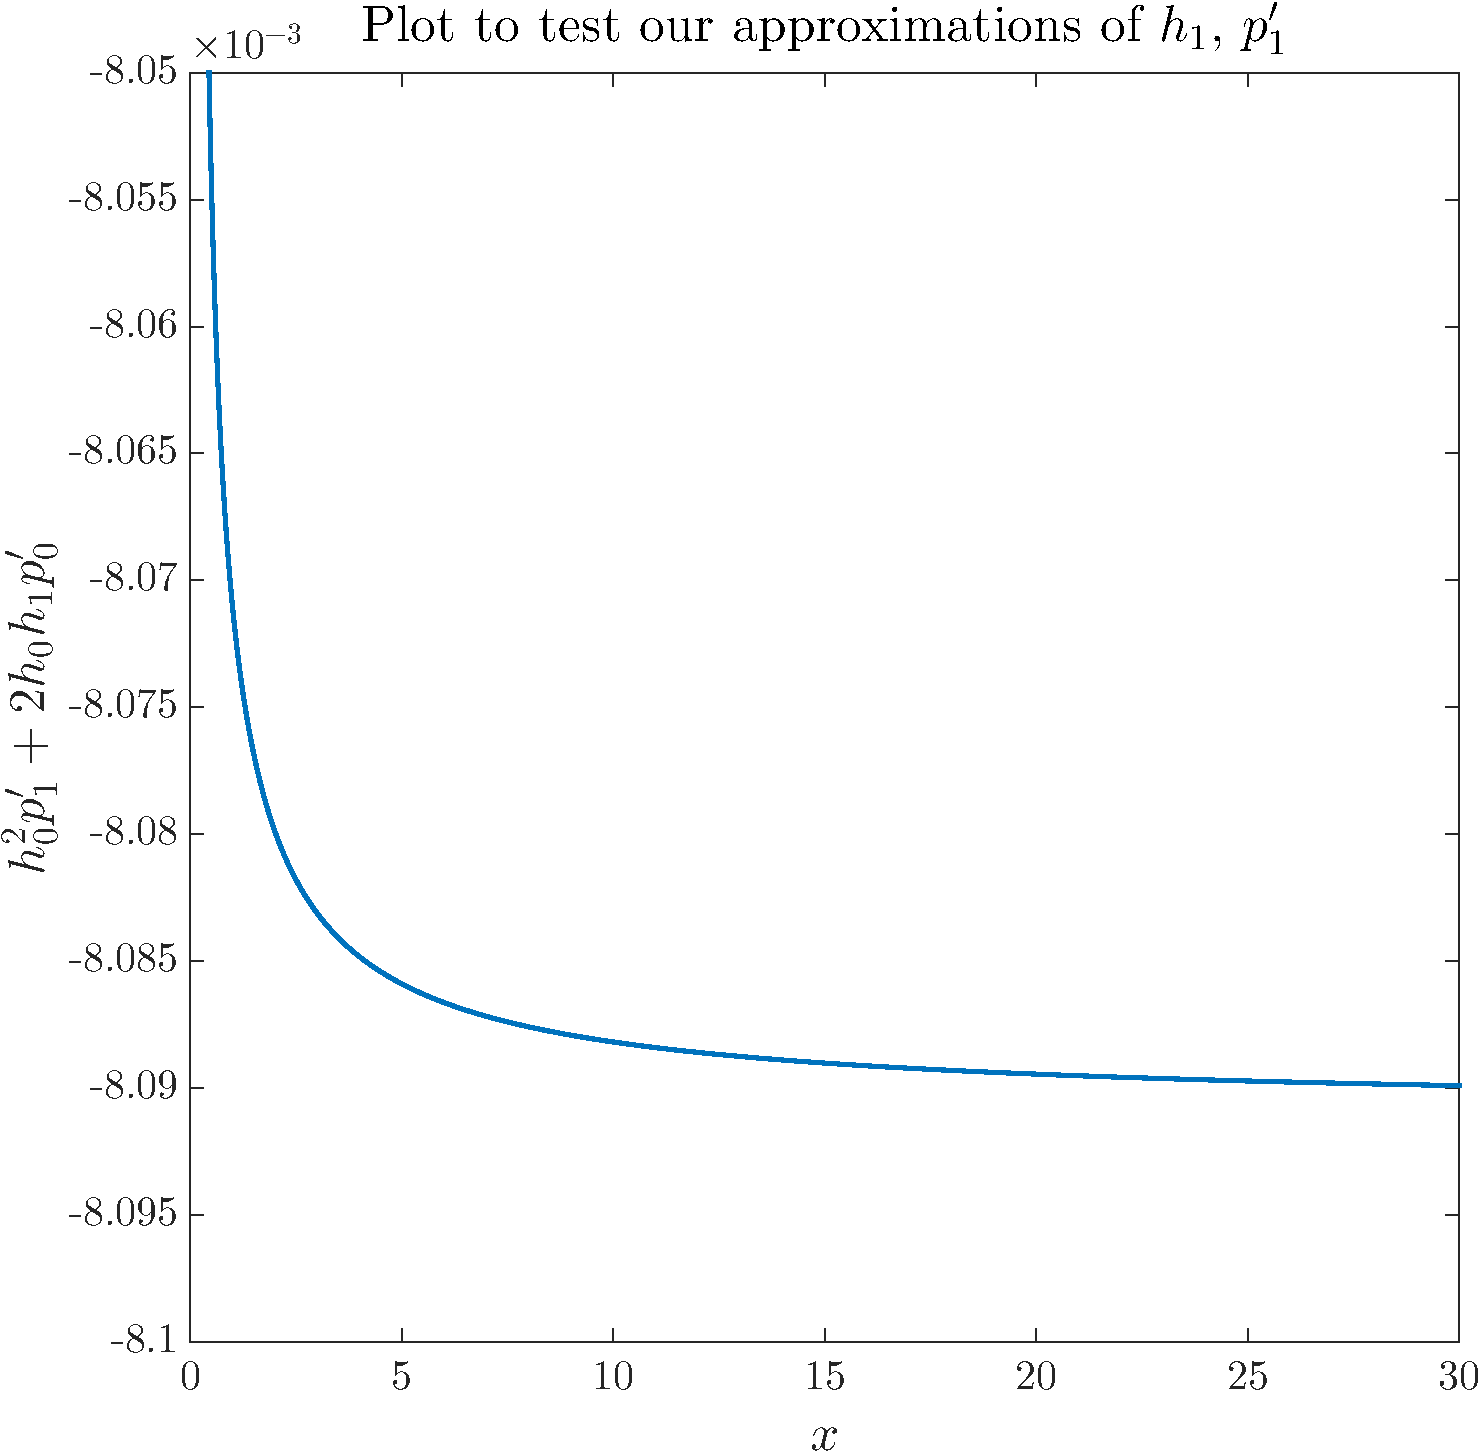
\includegraphics[scale=0.5]{linear-lubrication.pdf}
\end{figure}
%
\begin{figure}[!ht]\centering
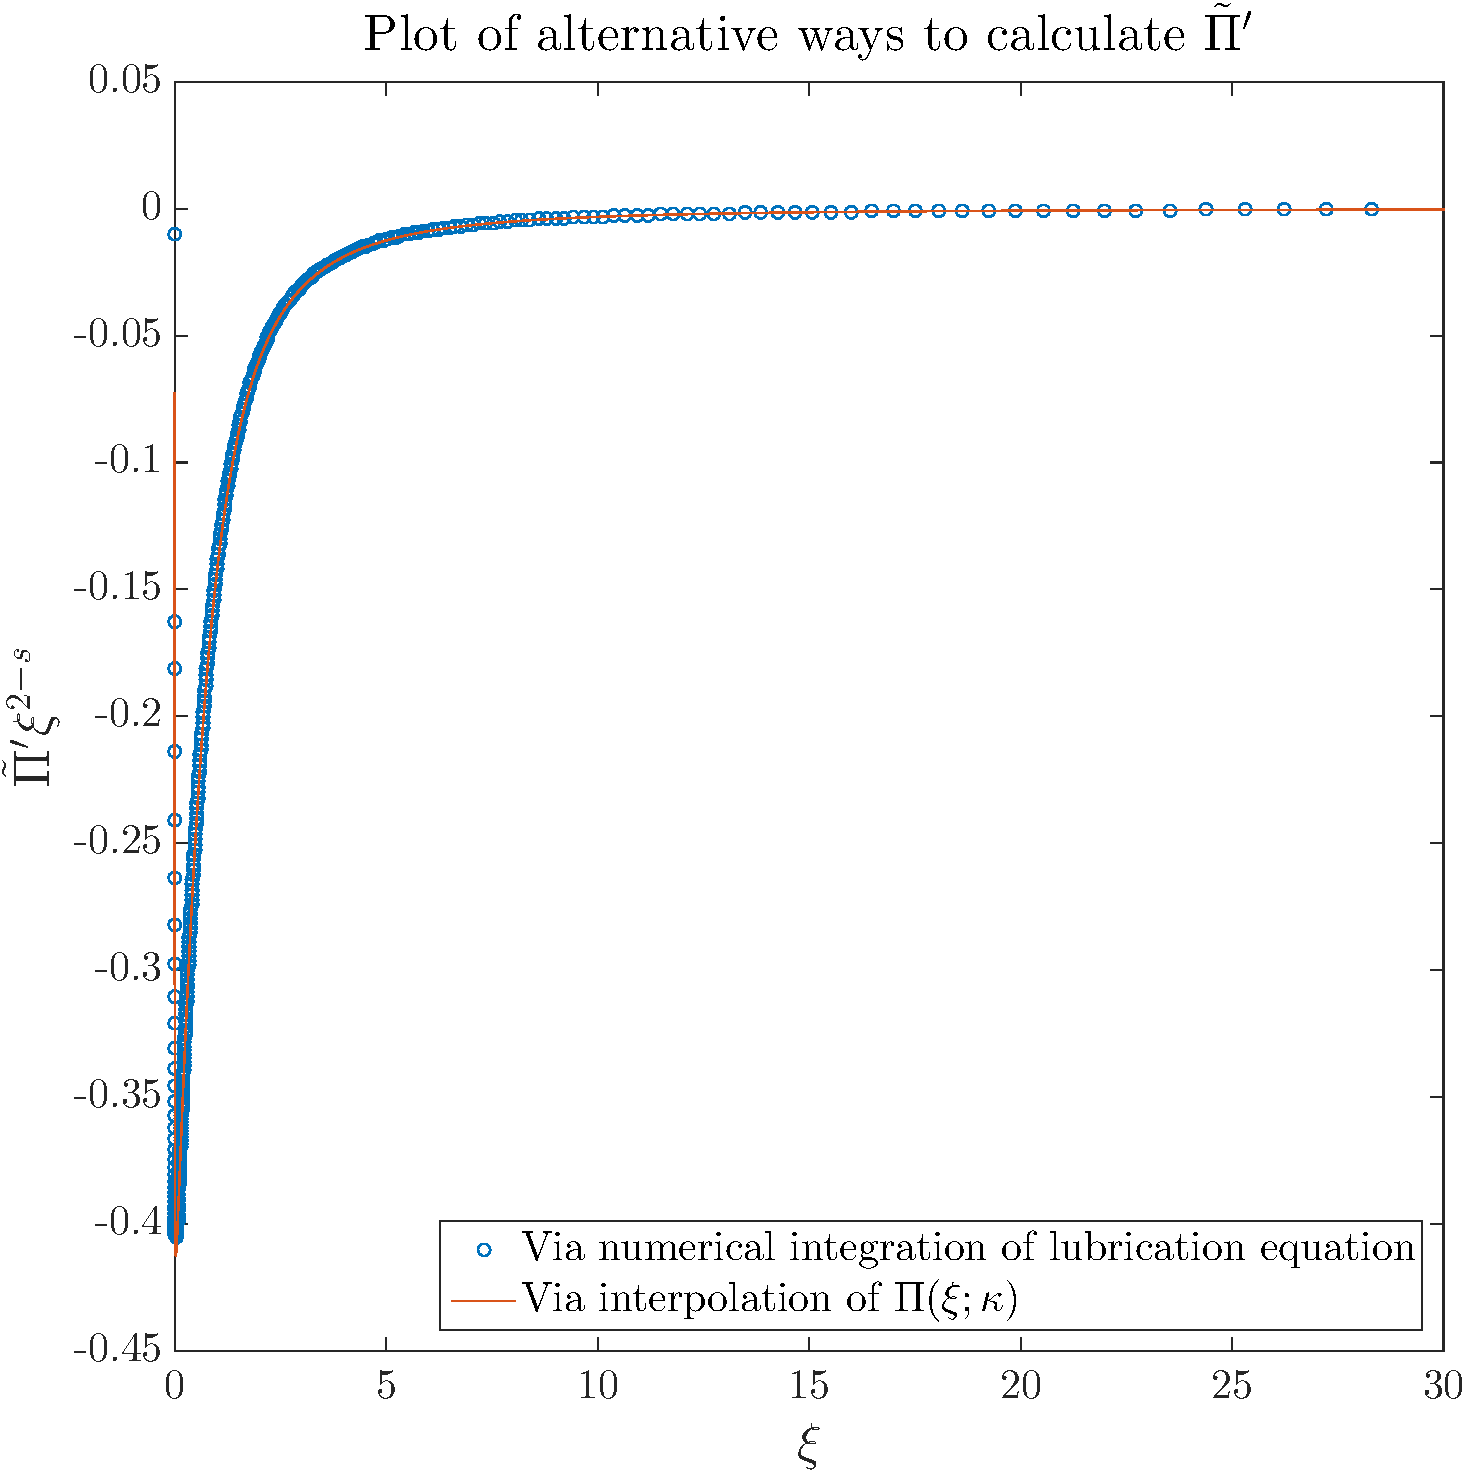
\includegraphics[scale=0.5]{Pi-prime.pdf}
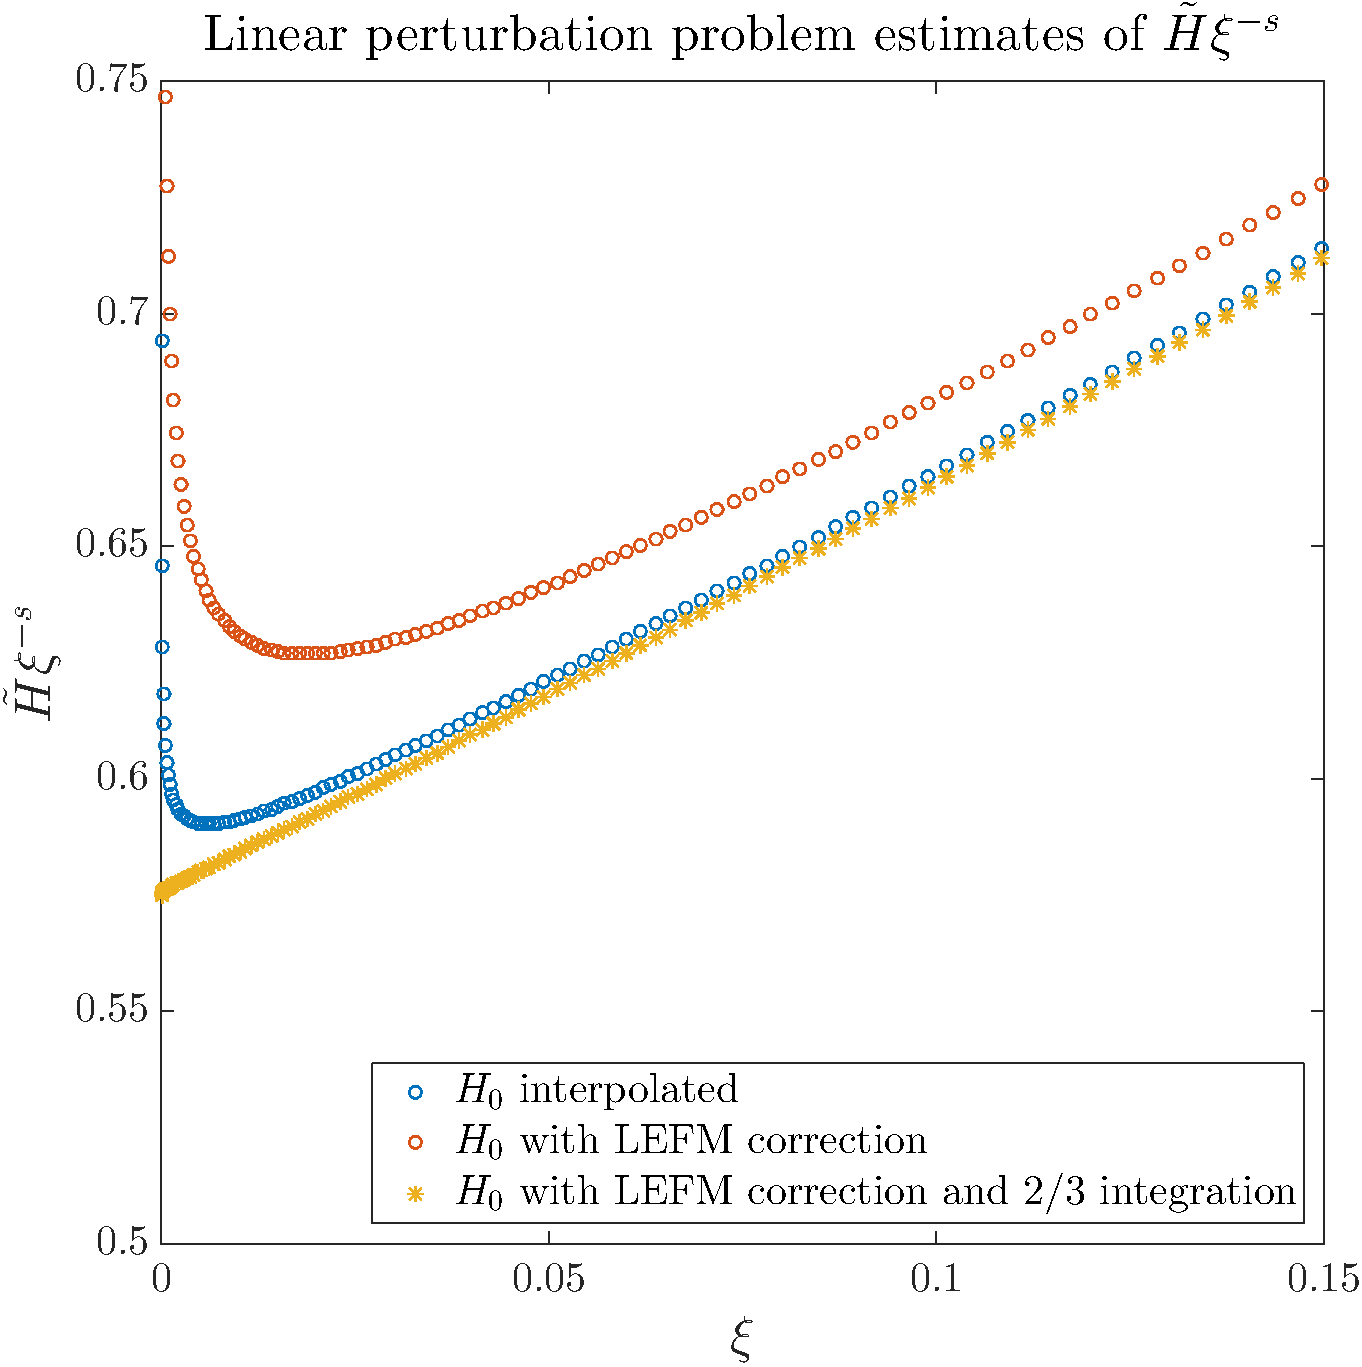
\includegraphics[scale=0.6]{linear-perturbation.pdf}
\end{figure}
\begin{figure}[!ht]\centering
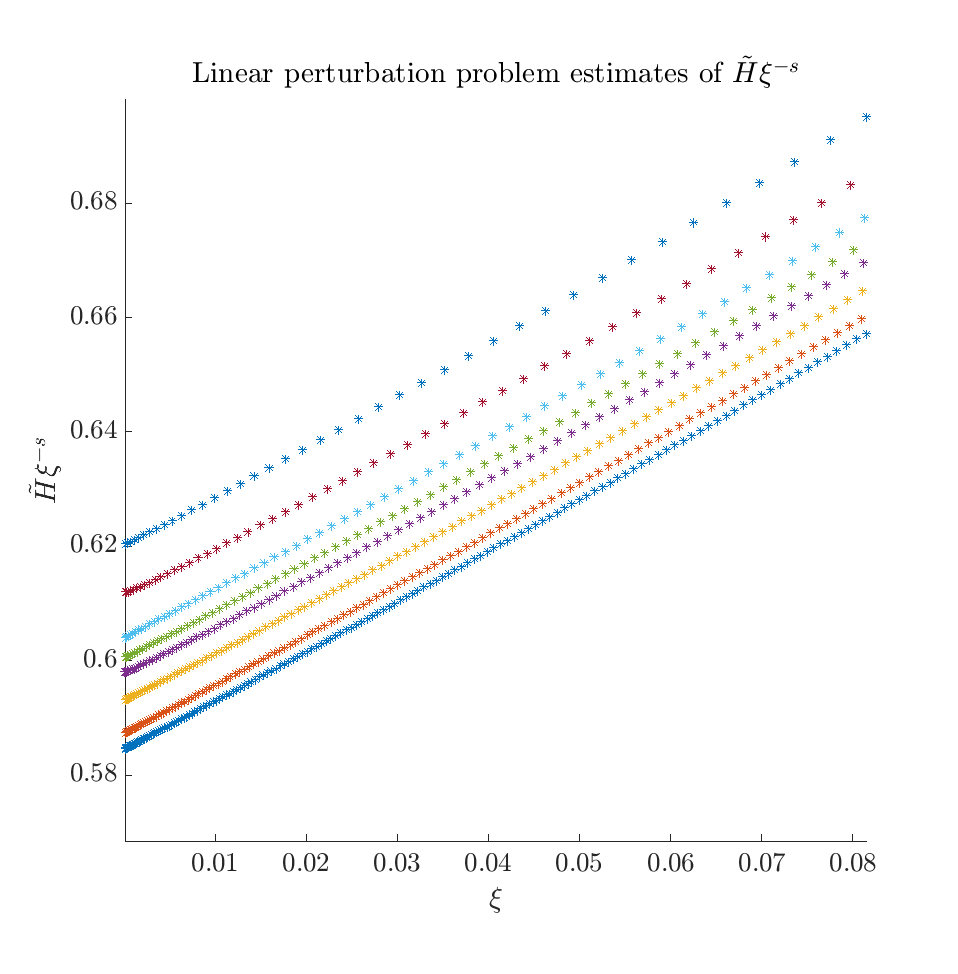
\includegraphics[scale=0.5]{linear-perturbation.png}
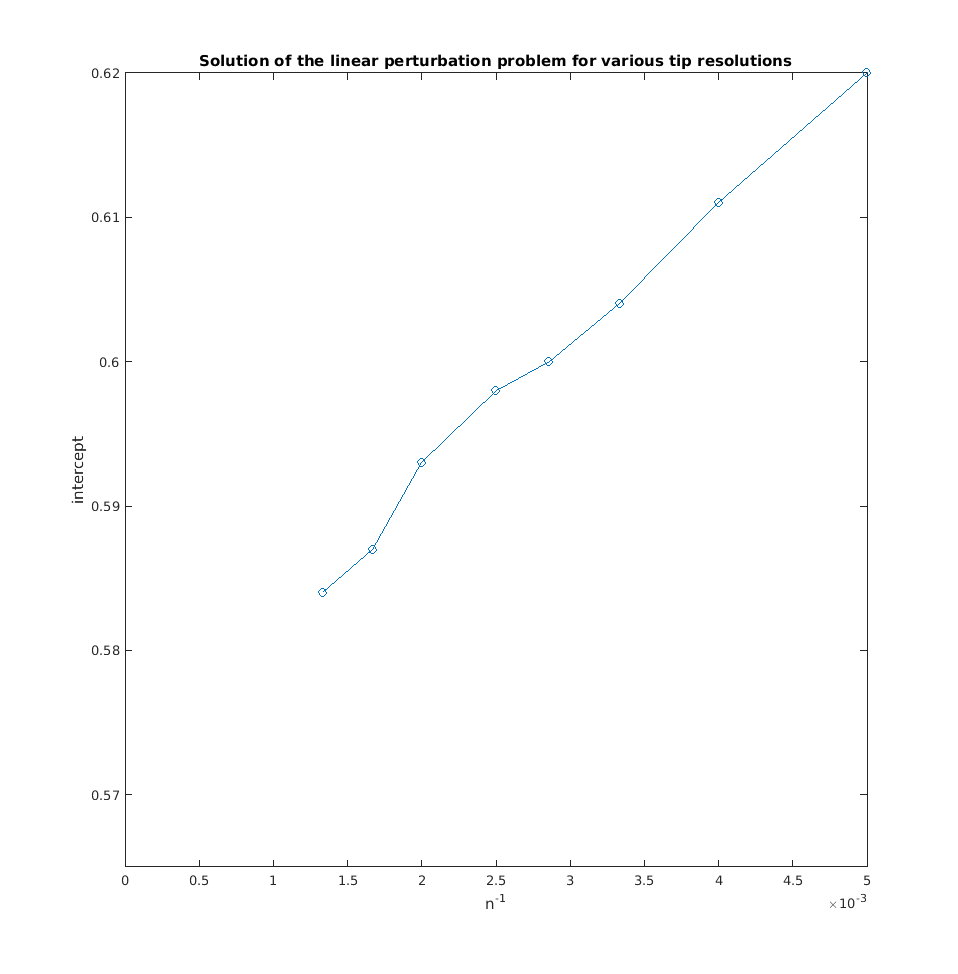
\includegraphics[scale=0.45]{resolution-effect.png}
\end{figure}
\begin{figure}[!ht]\centering
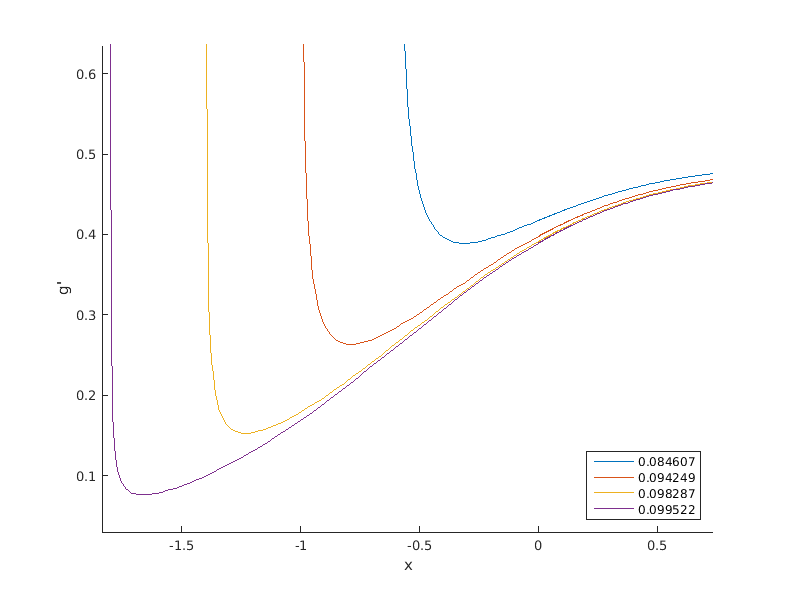
\includegraphics[scale=0.8]{gprime-variation.png}
\end{figure}

\end{document}
